\documentclass[10pt,a4paper]{article}

\usepackage[margin=2cm]{geometry}
\usepackage[T1]{fontenc}

\usepackage{graphicx}
\usepackage{booktabs}
\usepackage{caption}
\usepackage[hidelinks]{hyperref}

\graphicspath{{../figures/}}

\captionsetup{font=small}
\setlength{\parindent}{0pt}
\setlength{\parskip}{4pt}

\title{Chemical measurements and red wine quality}
\author{Jokubas Banaitis}
\date{15 October 2026}

\begin{document}

\maketitle
\vspace{-1.5em}

\section{Problem description and context}

This problem in question:
\textbf{Which chemical measurements are associated with
higher quality scores in red Vinho Verde wine?}

Laboratory measurements were compared with sensory scores,
focusing on alcohol and volatile acidity.

\section{Dataset and methods}

The red-wine subset of the UCI Wine Quality dataset contains
1,599 Portuguese red Vinho Verde wine observations,
11 physicochemical measurements, and one corresponding sensory
quality score~\cite{wine}. The dataset contains no missing values.

The scoring scale is 0 to 10, with scores 3--8 observed.
Alcohol: percentage by volume, Volatile acidity: acetic acid grams
per litre.

Python, pandas, and Matplotlib were used to read the
CSV file, count scores, calculate medians, and compute Spearman’s rank correlation.

\section{Overall results}

Scores 5 and 6 account for 1,319 observations (82.5\%).
Alcohol has the strongest absolute individual correlation
with quality ($\rho=0.479$), followed by volatile acidity
($\rho=-0.381$) and sulphates ($\rho=0.377$).

The small groups at scores 3 and 8 contain few observations, so their summaries are more sensitive to individual wines.


\begin{figure}[htbp]
    \centering

    \begin{minipage}{0.43\linewidth}
        \centering
        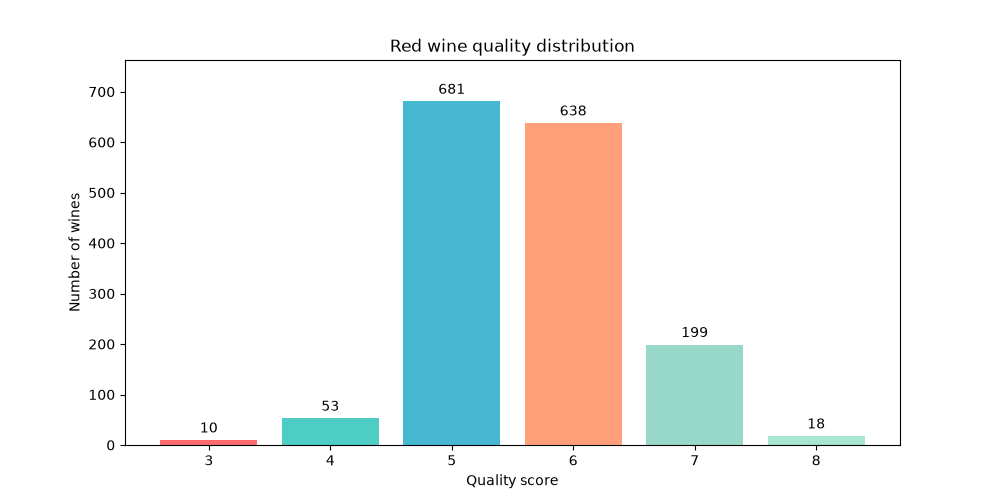
\includegraphics[width=\linewidth]{Figure_1.01.png}
    \end{minipage}
    \hfill
    \begin{minipage}{0.55\linewidth}
        \centering
        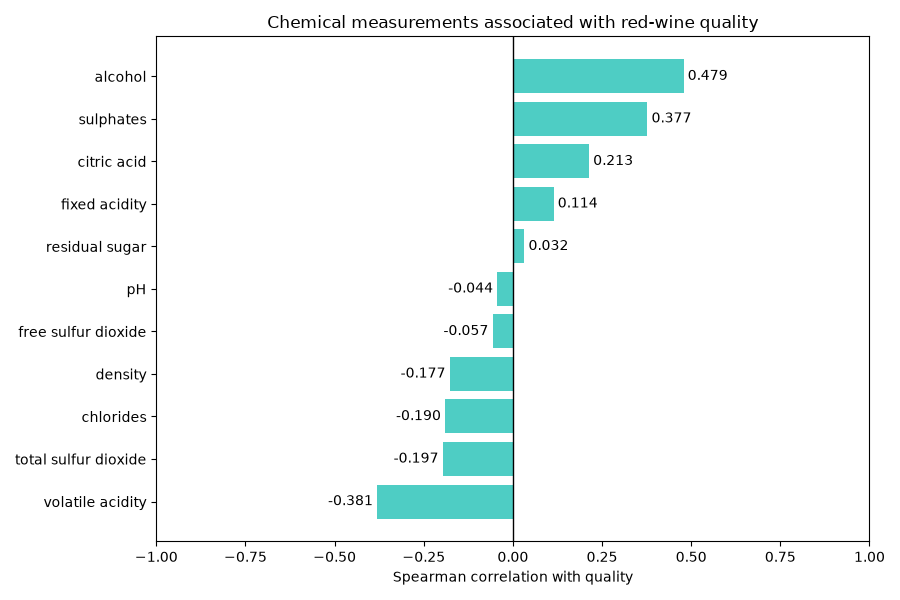
\includegraphics[width=\linewidth]{Figure_4.01.png}
    \end{minipage}

    \caption{Quality-score frequencies (left) and
    Spearman correlations with quality for all eleven
    chemical measurements (right).}
    \label{fig:overview}
\end{figure}

\clearpage

\section{Alcohol and volatile acidity by quality}

\begin{figure}[htbp]
    \centering
    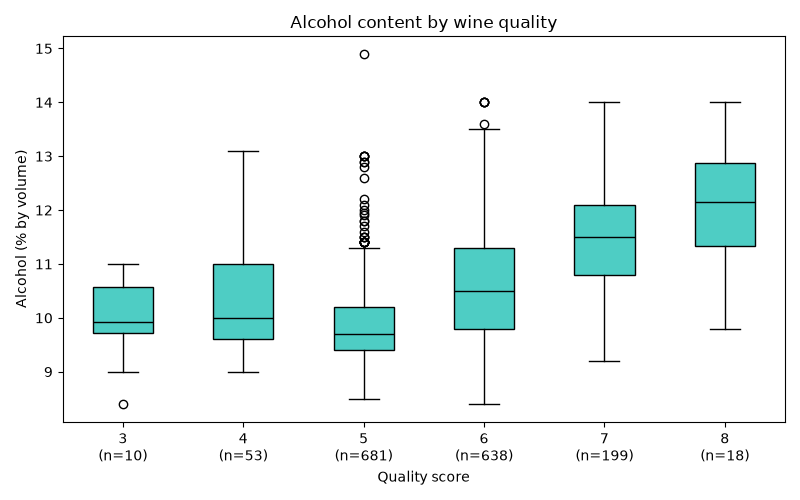
\includegraphics[width=0.68\linewidth]{Figure_2.01.png}

    \caption{Alcohol content by quality score.
    Median alcohol increases from 9.7\% at score 5
    to 11.5\% at score 7, but the distributions overlap.}
    \label{fig:alcohol}
\end{figure}

\begin{figure}[htbp]
    \centering
    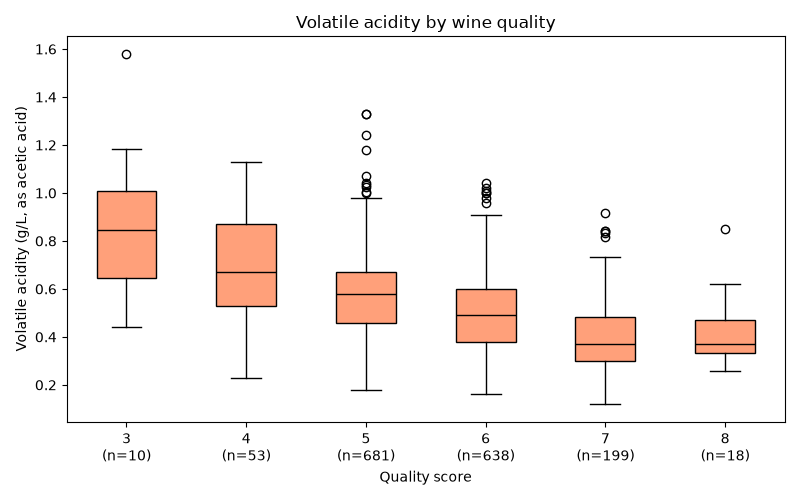
\includegraphics[width=0.68\linewidth]{Figure_3.01.png}

    \caption{Volatile acidity by quality score.
    The median decreases from 0.58 g/L at score 5
    to 0.37 g/L at score 7.}
    \label{fig:acidity}
\end{figure}

\small

In Figures~\ref{fig:alcohol} and~\ref{fig:acidity},
boxes contain the middle 50\% of measurements and
lines inside them indicate medians. The median was chosen because it is less influenced by extreme values when compared to the mean.

The interquartile range is
$\mathrm{IQR}=Q_3-Q_1$.
Whiskers reach the most extreme observations within
$Q_1-1.5\,\mathrm{IQR}$ and
$Q_3+1.5\,\mathrm{IQR}$.
Separate dots indicate observations beyond the scope.

\section{Conclusion and possible extension}

Between scores 5 and 7, median alcohol increases by
1.8 percentage points and median volatile acidity
decreases by 0.21 g/L.

The boxplots show differences in chemical units and
overlap that the correlations alone do not show. Higher alcohol content and lower volatile acidity can be associated with higher scores, although neither measurement provides a clear cutoff between
quality groups.

These results do not establish an ideal recipe. An "ideal" composition would also require experimental validation.

A future project could compare a training-median
baseline with models that use two or even all eleven
measurements, evaluated on wines excluded from training.

\begin{thebibliography}{1}

    \setlength{\itemsep}{0pt}

    \bibitem{wine}
    P. Cortez, A. Cerdeira, F. Almeida, T. Matos, and J. Reis (2009).
    \textit{Wine Quality}.
    UCI Machine Learning Repository.
    \href{https://doi.org/10.24432/C56S3T}
    {doi:10.24432/C56S3T}.
    Red subset, \texttt{winequality-red.csv}.
    Dataset licence: CC BY 4.0.

\end{thebibliography}

\end{document}